\iffalse
\def\mytitle{MATRICES USING PYTHON}
\def\myauthor{VAMSI SUNKARI}
\def\contact{vamsisunkari9849@gmail.com}
\def\mymodule{Future Wireless Communication (FWC)}
\documentclass[10pt, a4paper]{article}
\usepackage[a4paper,outer=1.5cm,inner=1.5cm,top=1.75cm,bottom=1.5cm]{geometry}
\twocolumn
\usepackage{graphicx}
\graphicspath{{./images/}}
\usepackage[colorlinks,linkcolor={black},citecolor={blue!80!black},urlcolor={blue!80!black}]{hyperref}
\usepackage[parfill]{parskip}
\usepackage{lmodern}
\usepackage{tikz}
 \usepackage{physics}
\usepackage{karnaugh-map}
\usepackage{setspace}
\doublespacing
%\documentclass{article}
\usepackage{tabularx}
%\usepackage{circuitikz}
\usetikzlibrary{calc}
\usepackage{amsmath}
\usepackage{amssymb}
\renewcommand*\familydefault{\sfdefault}
%\usepackage{watermark}
\usepackage{lipsum}
\usepackage{xcolor}
\usepackage{listings}
\usepackage{float}
\usepackage{titlesec}
\providecommand{\mtx}[1]{\mathbf{#1}}
\titlespacing{\subsection}{1pt}{\parskip}{3pt}
\titlespacing{\subsubsection}{0pt}{\parskip}{-\parskip}
\titlespacing{\paragraph}{0pt}{\parskip}{\parskip}
\newcommand{\figuremacro}[5]{
    \begin{figure}[#1]
        \centering
        \includegraphics[width=#5\columnwidth]{#2}
        \caption[#3]{\textbf{#3}#4}
        \label{fig:#2}
    \end{figure}
}
\newcommand{\myvec}[1]{\ensuremath{\begin{pmatrix}#1\end{pmatrix}}}
\let\vec\mathbf
\lstset{
frame=single, 
breaklines=true,
columns=fullflexible
}
\title{\mytitle}
\author{\myauthor\hspace{1em}\\\contact\\FWC22040\hspace{6.5em}IITH\hspace{0.5em}\mymodule\hspace{6em}ASSIGN-5}
\date{}
\begin{document}
 \maketitle
 \tableofcontents
   \section{Problem}
   \fi
   In Fig. 
		\ref{fig:9/9/4/5},
	\begin{figure}[!h]
		\centering
 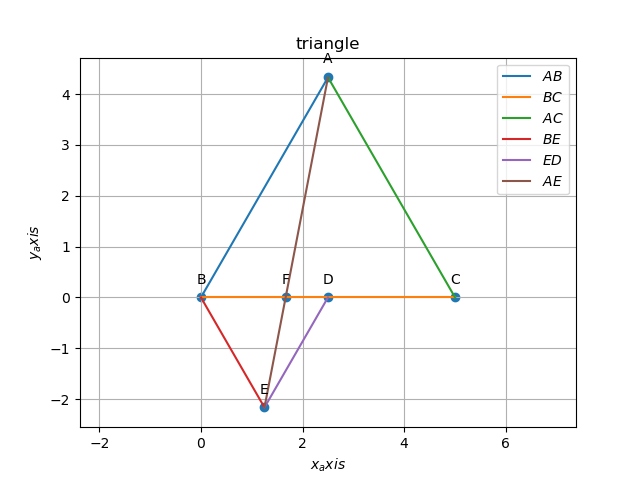
\includegraphics[width=\columnwidth]{chapters/9/9/4/5/figs/matrix.png}
		\caption{}
		\label{fig:9/9/4/5}
  	\end{figure}
$  ABC$ and $BDE$ are two equilateral
triangles such that $\vec{D}$ is the mid-point of $BC$. If $AE$
intersects $BC$ at $\vec{F}$, show that
\begin{align}
	ar(BDE) &=\frac{1}{4} ar(ABC)\\
	ar(BDE) &=\frac{1}{2} ar(BAE)\\
ar(ABC) &=2 ar(BEC)\\
ar(BFE) &= ar(AFD)\\
ar(BFE) &=2ar(FED)\\
	ar(FED) &=\frac{1}{8} ar(AFC)
\end{align}
\iffalse


\begin{proof}
From Appendix
    \ref{prop:two-isosc}, considering $\triangle$s $ABC$ and $EBD$,
\begin{align}
		\label{fig:9/9/4/5/b}
	\brak{\vec{B}-\vec{C}}^{\top}
	\brak{\vec{A}-\vec{D}} &=\vec{0}
	%\brak{\vec{A}-\frac{\vec{B}+\vec{C}}{2}}&=\vec{0}
	\\
	\brak{\vec{B}-\vec{D}}^{\top}
	\brak{\vec{E}-\frac{\vec{B}+\vec{D}}{2}}&=\vec{0}
		\label{fig:9/9/4/5/e}
\end{align}
		\eqref{fig:9/9/4/5/e}
		can be expressed as
\begin{align}
	\brak{\vec{B}-\vec{D}}^{\top}
	%\brak{\vec{B}-\brak{\frac{\vec{B}+\vec{C}}{2}}}^{\top}
	\brak{\vec{E}-\frac{\vec{B}+\vec{D}}{2}}&=\vec{0}
	%\brak{\vec{E}-\frac{\vec{B}+\brak{\frac{\vec{B}+\vec{C}}{2}}}{2}}&=\vec{0}
	\\
	\implies \brak{\vec{B}-\vec{C}}^{\top}
	\brak{\vec{E}-\frac{\vec{B}+\vec{D}}{2}}&=\vec{0}
%	\brak{\vec{E}-\frac{3\vec{B}+2\vec{C}}{2}}&=\vec{0}
		\label{fig:9/9/4/5/e/2}
\end{align}
upon substituting
\begin{align}
	\vec{D}=\frac{\vec{B}+\vec{C}}{2}
\end{align}
From 
		\eqref{fig:9/9/4/5/b},
		\eqref{fig:9/9/4/5/e/2}
		and 
	  Appendix \ref{prop:two-orth-para},
\begin{align}
	\vec{E}-\frac{\vec{B}+\vec{D}}{2}&=
	k\brak{\vec{A}-\vec{D}}
	%\vec{E}-\frac{3\vec{B}+2\vec{C}}{2}&=
	%k\brak{\vec{A}-\brak{\frac{\vec{B}+\vec{C}}{2}}}
	\\
\implies
	\vec{E} &= \frac{\vec{B}+\vec{D}}{2}+k\brak{\vec{A}-\vec{D}}
	%\frac{3\vec{B}+2\vec{C}}{2}+	k\brak{\vec{A}-\brak{\frac{\vec{B}+\vec{C}}{2}}}
	%\vec{E} &= \frac{3\vec{B}+2\vec{C}}{2}+	k\brak{\vec{A}-\brak{\frac{\vec{B}+\vec{C}}{2}}}
		\label{fig:9/9/4/5/ef}
\end{align}
Since
\begin{align}
	\vec{E} \times \vec{B} &=\frac{\vec{D}\times \vec{B}}{2}+k\brak{\vec{A}-\vec{D}} \times \vec{B}
	\\
	&=\brak{\frac{1}{2}-k}\vec{D}\times \vec{B}+k\vec{A} \times \vec{B}
	%\vec{E} \times \vec{B} &=\brak{\frac{3\vec{B}+2\vec{C}}{2}+k\brak{\vec{A}-\brak{\frac{\vec{B}+\vec{C}}{2}}}} \times \vec{B}
%	\\
%	&=\brak{\vec{C}+k\brak{\vec{A}-\brak{\frac{\vec{C}}{2}}}} \times \vec{B}
%	\\
%	\vec{B} \times \vec{D} &=\vec{B} \times \frac{\vec{B}+\vec{C}}{2}
%	\\
%	&=\vec{B} \times \frac{\vec{C}}{2}
	\\
	\vec{D} \times \vec{E}&=\frac{\vec{D}\times\vec{B}}{2}+k \vec{D}\times\vec{A}
	%\vec{D} \times \vec{E}&=\brak{\frac{\vec{B}+\vec{C}}{2}}\times\brak{\frac{3\vec{B}+2\vec{C}}{2}+	k\brak{\vec{A}-\brak{\frac{\vec{B}+\vec{C}}{2}}}}
\end{align}
	upon substituting from 
		\eqref{fig:9/9/4/5/ef},
\begin{align}
		\label{fig:9/9/4/5/e/area}
{\vec{E} \times \vec{B}+\vec{B} \times \vec{D}+\vec{D} \times \vec{E}}
 \\
= 
k\brak{\vec{A} \times \vec{B}+\vec{B} \times \vec{D}+\vec{D} \times \vec{A}}
%	\\
%	+\vec{B} \times \vec{D}+\vec{D} \times \brak{\frac{3\vec{B}+2\vec{C}}{2}+k\brak{\vec{A}-\brak{\frac{\vec{B}+\vec{C}}{2}}}}
\end{align}
%upon  substituting from 
%		\eqref{fig:9/9/4/5/ef}
		%in
		%\eqref{fig:9/9/4/5/e/area},
\end{proof}
%\iffalse
From 
	  \eqref{eq:two-tri-indep},
\begin{align}
	  \brak{p+q}\vec{E}- p\vec{B} -q\vec{D} &= 0
	  \\
	  \implies
	  \brak{p+q}\brak{\frac{\vec{B}+\vec{D}}{2}+k\brak{\vec{A}-\vec{D}}}- p\vec{B} -q\vec{D} &= 0
	  \\
	  \text{or, }
	  \brak{\frac{q-p}{2}}\vec{B}+\brak{\frac{p-q}{2}-k\brak{p+q}}\vec{D}+k\vec{A}&= 0
\end{align}
Since $\vec{D}$ is the mid point of $BC$, substituting 
in the above,
\begin{align}
	\brak{\frac{q-p}{2}}\vec{B}+\brak{\frac{p-q}{2}-k\brak{p+q}}\brak{\frac{\vec{B}+\vec{C}}{2}}+k\vec{A}&= 0
%	\brak{\frac{q-p}{2}}\vec{B}-\brak{q+k\brak{{\frac{p+q}{2}}}}\frac{\vec{B}+\vec{C}}{2}+k\brak{p+q}\vec{A}&= 0
%	  \\
%	  \implies
%k\brak{p+q}\vec{A}+
%	\brak{\frac{q-p}{2}-\brak{q+k\brak{{\frac{p+q}{2}}}}}\vec{B}-\brak{q+k\brak{{\frac{p+q}{2}}}}\frac{\vec{B}+\vec{C}}{2}+k\brak{p+q}\vec{A}&= 0
	\\
	\implies 
	k\vec{A}+\brak{\frac{q-p}{2}}\vec{B}+\brak{\frac{p-q}{2}-k\brak{p+q}}\brak{\frac{\vec{B}+\vec{C}}{2}}&= 0
\end{align}
in the above, 

[Hint : Join EC and AD. Show that BE  AC abd DE AB, etc.]

   %  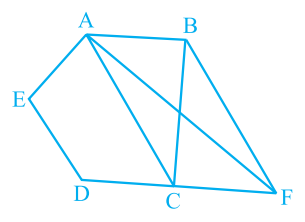
\includegraphics[scale=1.0]{diag_1.png}
   \section{Solution}
   \textbf{Theory:}\\
   \textbf{To Prove:} ar(BDE)=1/4 ar(ABC) \\
   ABC and BDE are two equilateral triangles such that D is the mid-point of BC.If AE intersets BC at F


\textbf{termux commands :}
\begin{lstlisting}
python3 matrix.py
\end{lstlisting}


The input parameters for this construction are 
\begin{center}
\begin{tabular}{|c|c|c|}
 \hline
 \textbf{Symbol}&\textbf{Value}&\textbf{Description}\\
 \hline
 r&5&AB\\
 \hline

 $\vec{A}$&$r\myvec{\cos\theta \\ \sin\theta}$%
 &Point A\\
 \hline
 $\vec{E}$&$\myvec{\frac{r}{2}\cos\theta \\ \frac{r}{2}\sin\theta}$
 &Point E\\
 \hline
 $\vec{B}$&$\myvec{0 \\ 0}$%
 &Point B\\
 \hline
 $\vec{C}$&$\myvec{r \\ 0}$%
 &Point C\\
 \hline
 $\vec{D}$&$\myvec{r/2 \\ 0}$%
 &Point D\\
 \hline
 $\vec{F}$&$\myvec{\frac{2}{3}r\cos\theta \\ 0}$%
 &Point F\\
 \hline
 ${\theta}_1$& $\pi/3$&$ \angle $ABC\\ 
 \hline
\end{tabular}
\end{center}
\textbf{To Prove:} ar(BDE)=1/4 ar(ABC)
  \begin{center}
 
 $\vec{v1}=\vec{A-B}$\\
 $\vec{v2}=\vec{A-C}$\\

$ar(\Delta ABC) =\frac{1}{2}\norm{\vec{v1}\times\vec{v2}}$............(1)\\
$\vec{v3}=\vec{B-D}$\\
 $\vec{v4}=\vec{B-E}$\\
 
 $ar(\Delta BDE) =\frac{1}{2}\norm{\vec{v3}\times\vec{v4}}$...............(2)\\
 $ar(BDE)= \frac{1}{4} ar(ABC)$
 \end{center}
 \textbf{To Prove:}  ar(BDE)=1/2 ar(BAE) 
 \begin{center}
$\vec{v5}=\vec{A-E}$\\
$\vec{v6}=\vec{A-B}$\\

 $ar(\Delta BAE) =\frac{1}{2}\norm{\vec{v5}\times\vec{v6}}$...............(3)\\
 $ar(BDE)=\frac{1}{2} ar(BAE)$
\end{center}
 \textbf{To Prove:}  ar(ABC)=2 ar(BEC) 
 \begin{center}
 $\vec{v7}=\vec{B-C}$\\
$\vec{v8}=\vec{B-E}$\\

 $ar(\Delta BEC) =\frac{1}{2}\norm{\vec{v7}\times\vec{v8}}$...............(4)\\
 $ar(ABC)=2 ar(BEC)$
 \end{center}
 \textbf{To Prove:}  ar(BFE)=ar(AFD) 
 \begin{center}
 $\vec{v9}=\vec{B-F}$\\
$\vec{v10}=\vec{B-E}$\\
$\vec{v11}=\vec{A-D}$\\
$\vec{v12}=\vec{A-F}$\\
 $ar(\Delta BFE) =\frac{1}{2}\norm{\vec{v9}\times\vec{v10}}$...............(4)\\
 $ar(\Delta AFD) =\frac{1}{2}\norm{\vec{v11}\times\vec{v12}}$...............(4)\\
 ar(BFE)=ar(AFD)
 \end{center}
 \textbf{To prove} : ar(BFE) =2ar(FED)
\begin{center}
$\vec{v13}=\vec{F-E}$\\
$\vec{v14}=\vec{F-D}$\\
 $ar(\Delta FED) =\frac{1}{2}\norm{\vec{v13}\times\vec{v14}}$...............(4)\\
 $ar(BFE) =2ar(FED)$   
\end{center}
\textbf{To prove} : $ar(FED) =\frac{1}{8} ar(AFC)$
\begin{center}
$\vec{v15}=\vec{A-F}$\\
$\vec{v16}=\vec{A-C}$\\
$ar(\Delta AFC) =\frac{1}{2}\norm{\vec{v15}\times\vec{v16}}$...............(4)\\ 
 $ar(FED) =\frac{1}{8} ar(AFC)$   
\end{center}
The below python code realizes the above construction: 
\begin{lstlisting}
https://github.com/Vamsi9849/iithfwc/blob/main/Matrix_line/codes/matrix.py
\end{lstlisting}
 \section{Construction}
  \begin{center}
  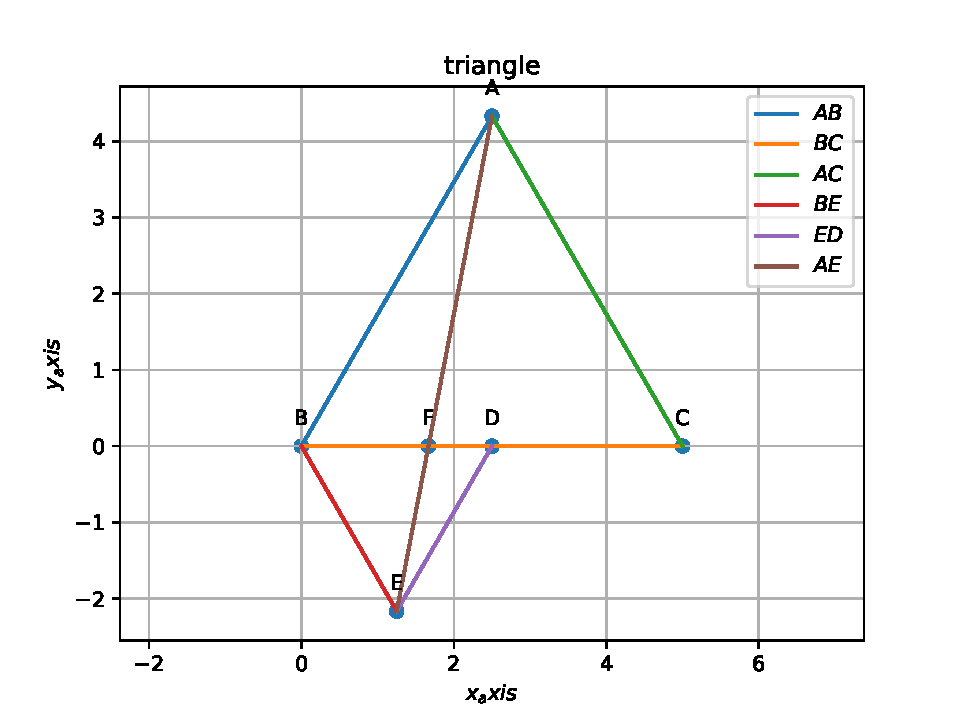
\includegraphics[scale=0.39]{par.pdf}  
  Figure of construction
   \end{center}   
\bibliographystyle{ieeetr}
\end{document}
\fi
